\section{Synchronization}
\subsection*{Critical Section (CS)}
\emph{Properties:} Mutual exclusion, progress(if no process in CS, waiting process evetually granted access), bounded wait.\\
\emph{Assumptions:} independence on non-CS, takes finite time.\\
\emph{Problems:} Deadlock, starvation, livelock(keeping changing state with no progress).

\subsection*{Peterson's Algorithm}
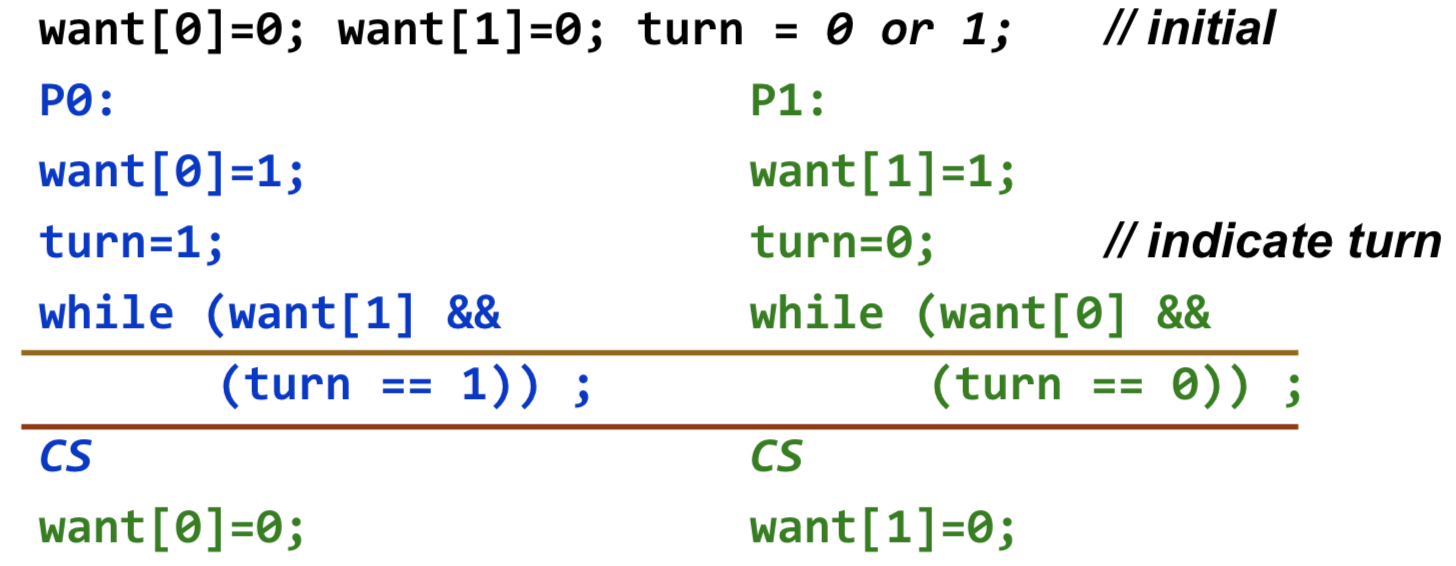
\includegraphics[width=0.6\linewidth]{images/peterson-algo} (-) busy waiting
 
\subsection*{Semaphore}
\emph{Wait() and Signal():}\\
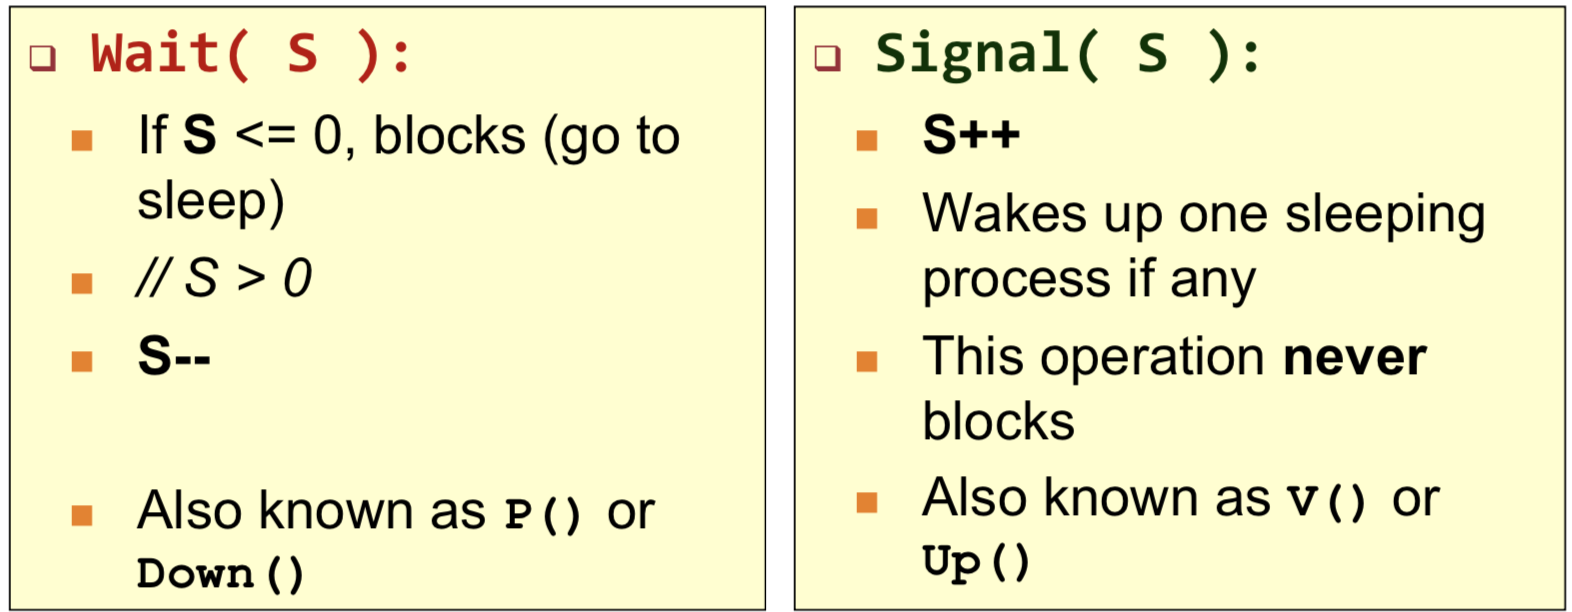
\includegraphics[width=0.75\linewidth]{images/wait-and-signal}\\
$S_{curr}=S_{init}+\#signal(S)-\#wait(S\_comp)$\\
\emph{Mutex:} S=1; Wait(S); CS; Signal(S).

\subsection*{Classic Synchronization Problems}
\emph{Producer Consumer (Blocking):}\\
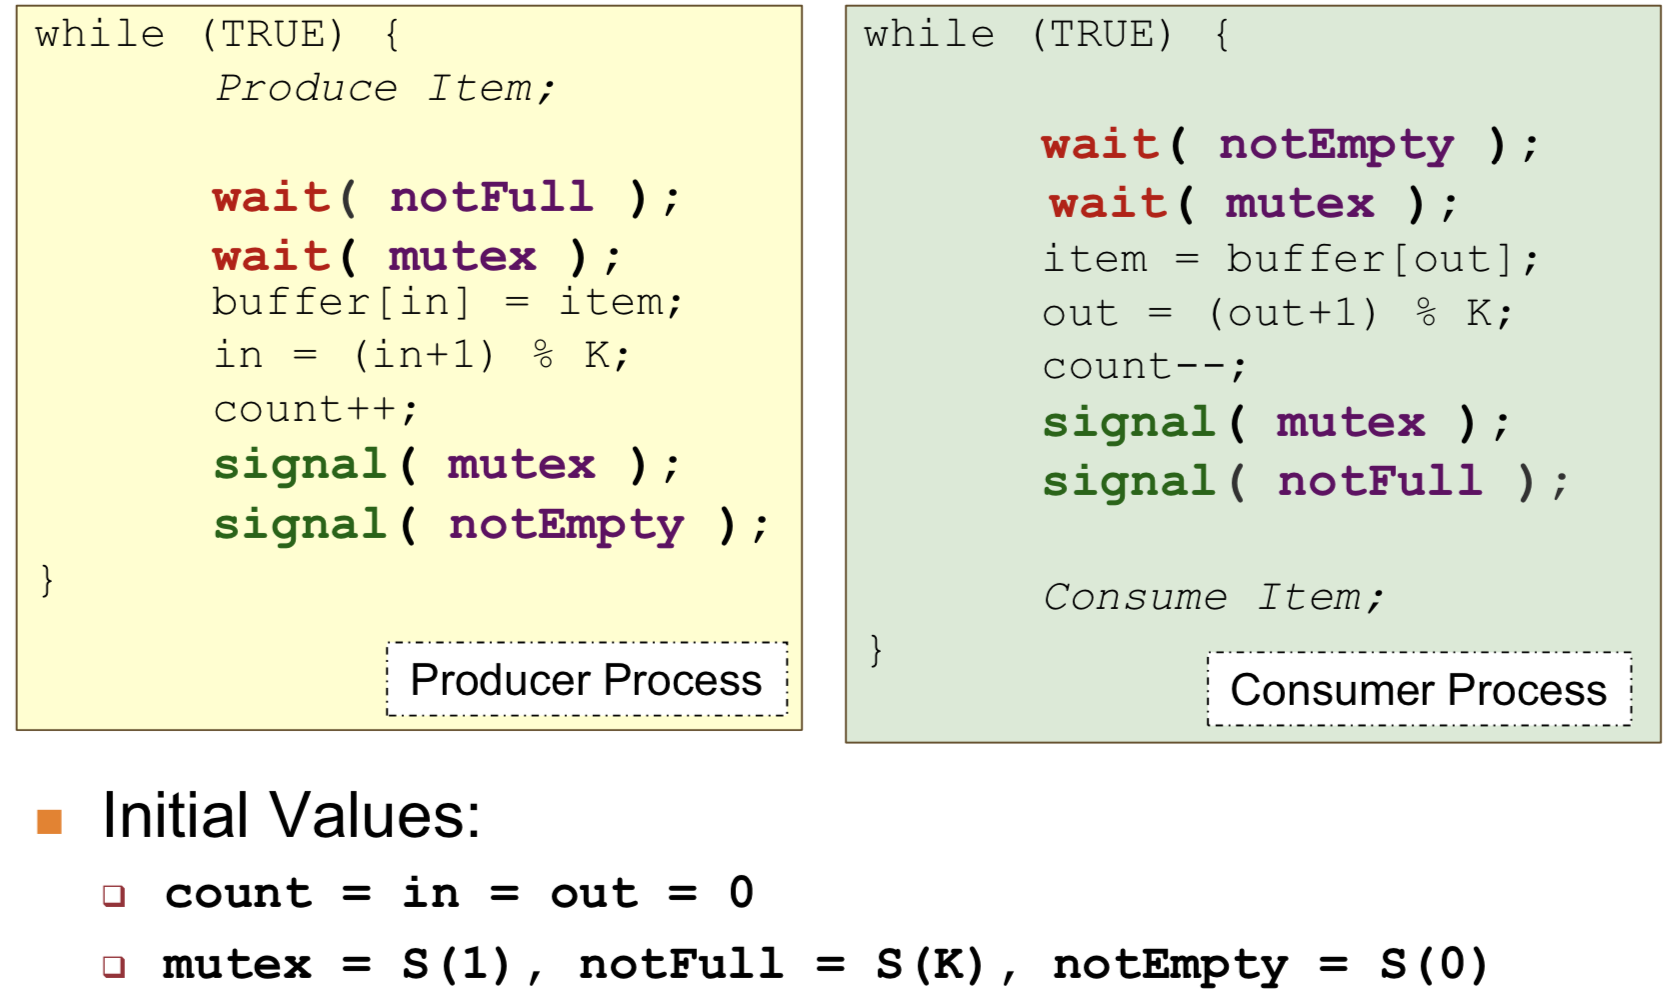
\includegraphics[width=0.75\linewidth]{images/producer-consumer}\\
\emph{Reader Writer:}\\
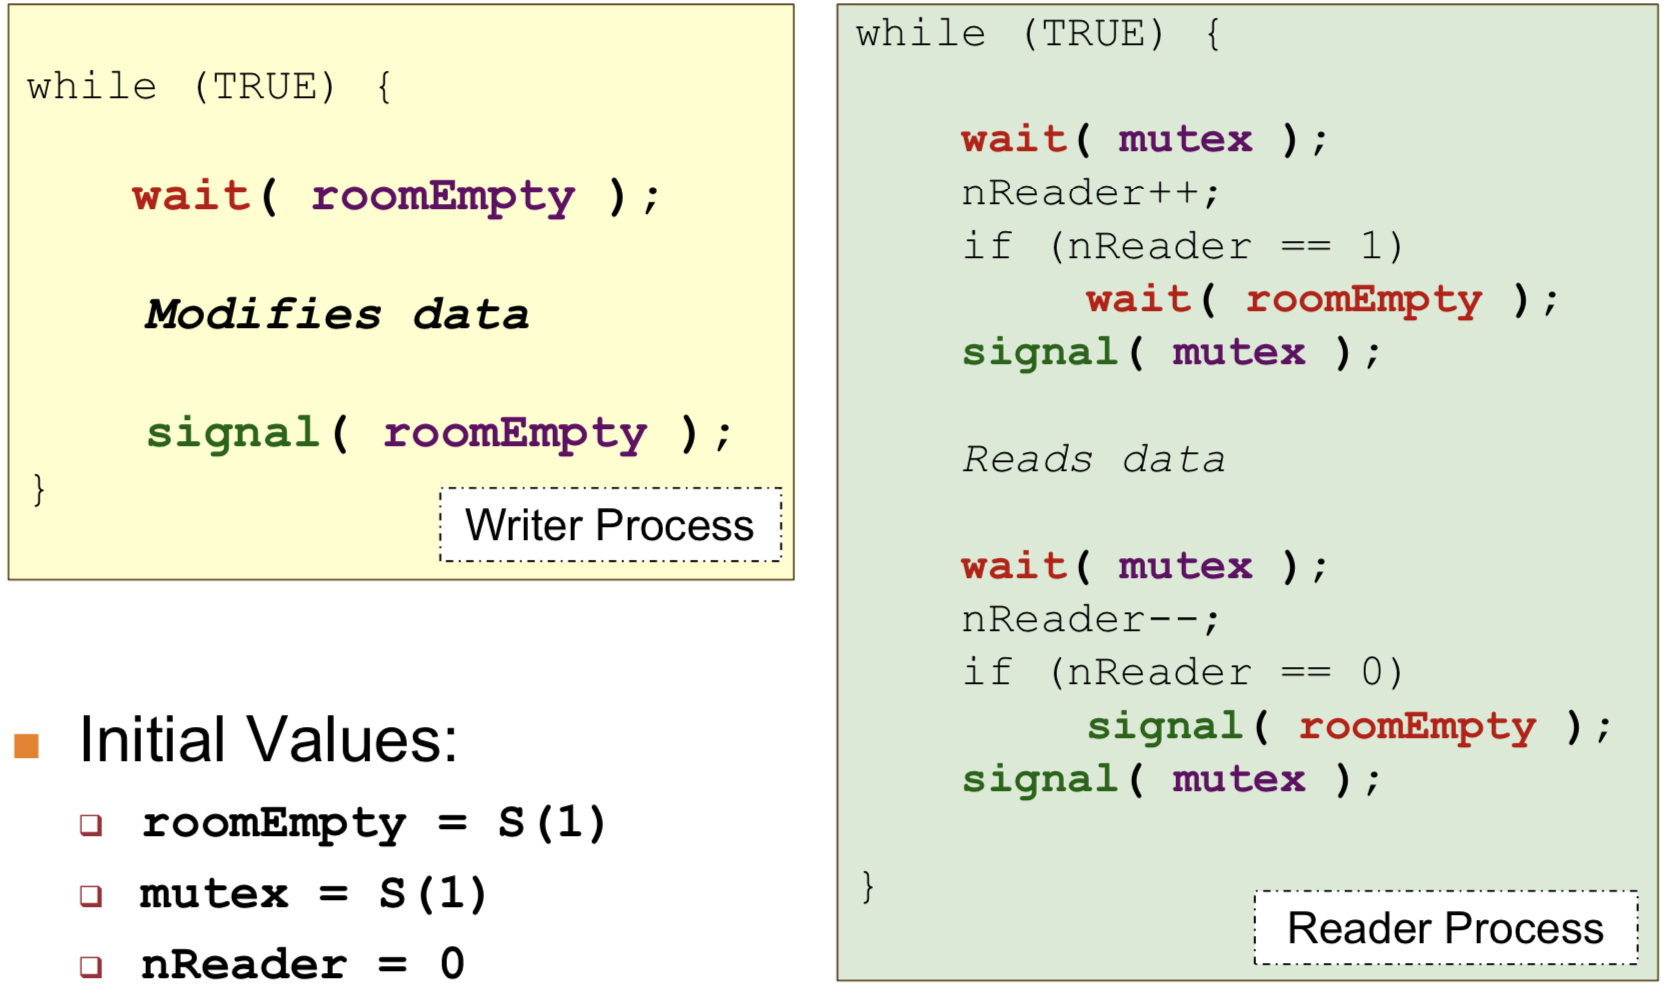
\includegraphics[width=0.75\linewidth]{images/reader-writer}\\
\emph{Dinning Philosopher:}\\
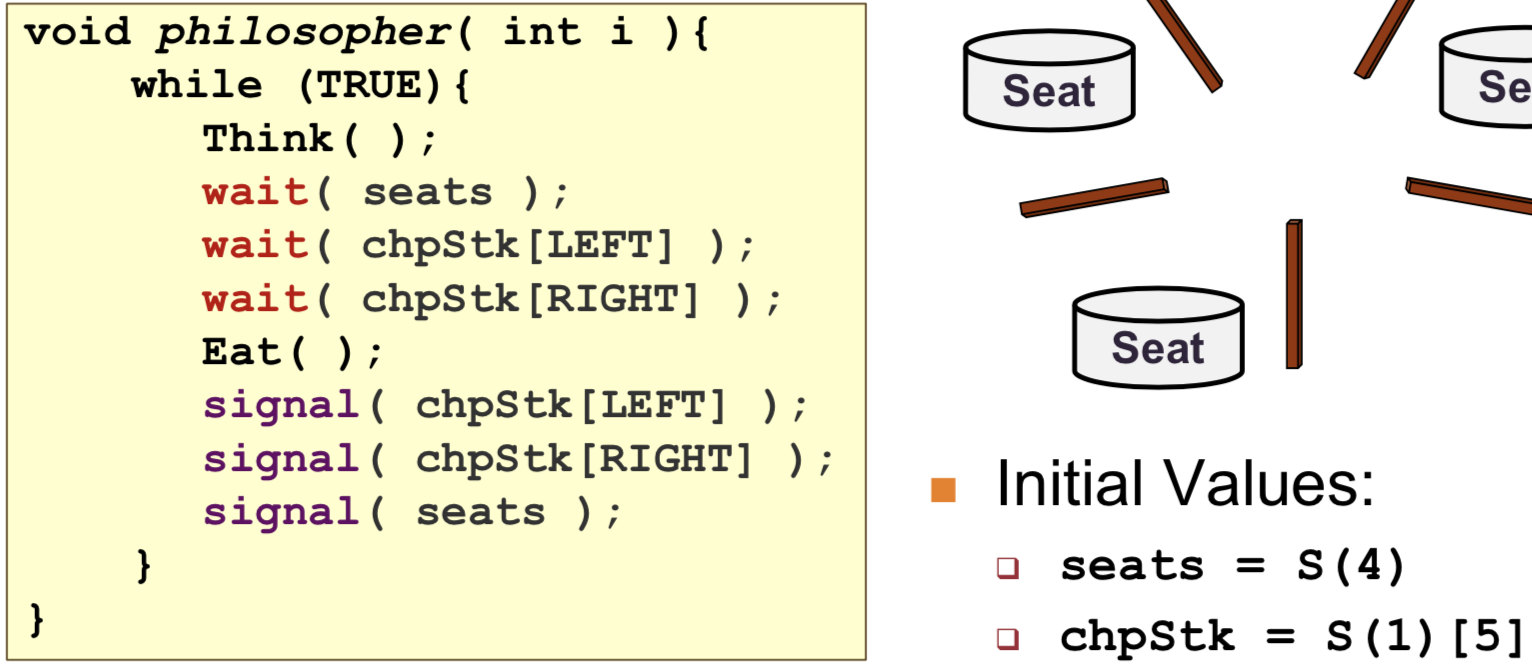
\includegraphics[width=0.75\linewidth]{images/philo-limited-eater}

\subsection *{OS Implementation}
\emph{User mode semaphore implemted by OS:}\\
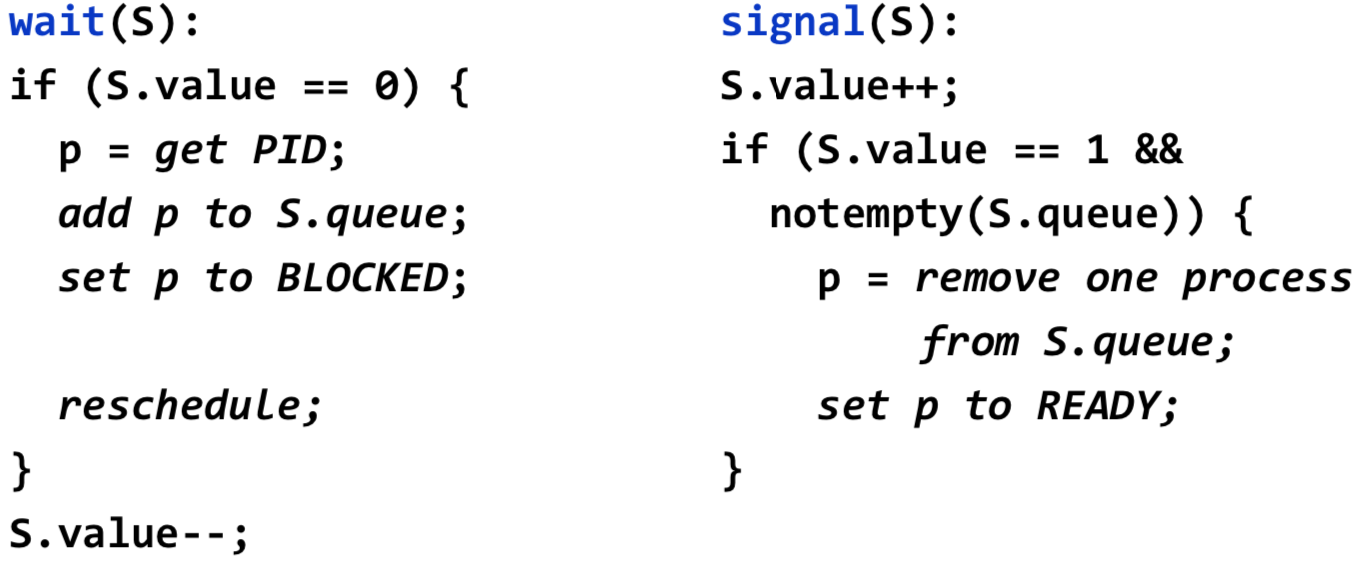
\includegraphics[width=0.75\linewidth]{images/user-semaphore}\\
\emph{Kernel:} disable interrupt(miss interrupt, interfere scheduling)\\
\emph{Multi-processor:} Busy-waiting mutual exclusion(spinlock), HW with atomic read+write\\
\emph{Hardware atomic instruction:} TestAndSet\\
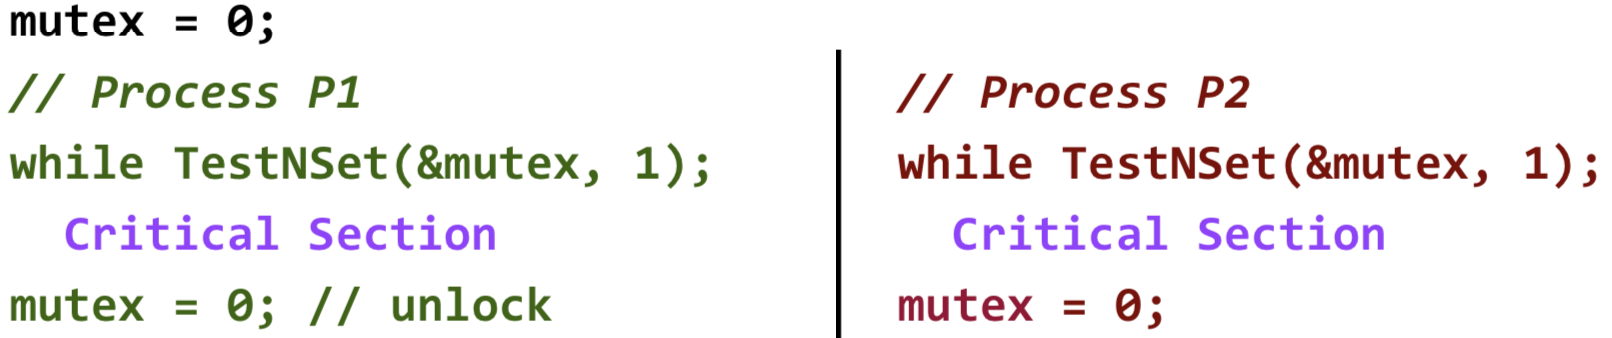
\includegraphics[width=0.7\linewidth]{images/test-and-set} (spinlock)